%%%%%%%%%%%%%%%%%%%%%%%%%%%%%%%%%%%%%%%%%%%%%%%%%%%%%%%%%%%%%%%%%%%%%%%%
% 
% LaTeX Template
%
%%%%%%%%%%%%%%%%%%%%%%%%%%%%%%%%%%%%%%%%%%%%%%%%%%%%%%%%%%%%%%%%%%%%%%%%

%------------------------------------------------------------------------------------------------
%	DOCUMENT CONFIGURATIONS
%------------------------------------------------------------------------------------------------

% DOCUMENT
%   - Properties
\documentclass[a4paper,11pt]{report} % Sets a two-sided A4 sized paper.
                                         % (Two-sided for LaTeX to distinguish between odd/even
                                         % pages while using headers and footers.)
\linespread{1.15}                         % Default space between lines
                                    % Margin sizes defined in headers_and_footers file.
\usepackage[nottoc,numbib]{tocbibind}    % Makes References section appear in the Table of contents (nottoc). Conuts the References like section.
\usepackage{lastpage}                    % To get the total number of pages.

%   - Sectioning
\usepackage{titlesec}                   % Extra features for sectioning
    % The following lines create: \subsubsubsection{}
    
    
%%%%%%%%% From here: creation of \subsubsubsection{} %%%%%%%%%
    \titleclass{\subsubsubsection}{straight}[\subsection]

    \newcounter{subsubsubsection}[subsubsection]
    \renewcommand\thesubsubsubsection{\thesubsubsection.\arabic{subsubsubsection}}
    \renewcommand\theparagraph{\thesubsubsubsection.\arabic{paragraph}} % optional; useful if paragraphs are to be numbered

    \titleformat{\subsubsubsection}
      {\normalfont\normalsize\bfseries}{\thesubsubsubsection}{1em}{}
    \titlespacing*{\subsubsubsection}
    {0pt}{3.25ex plus 1ex minus .2ex}{1.5ex plus .2ex}

    \makeatletter
    \renewcommand\paragraph{\@startsection{paragraph}{5}{\z@}%
      {3.25ex \@plus1ex \@minus.2ex}%
      {-1em}%
      {\normalfont\normalsize\bfseries}}
    \renewcommand\subparagraph{\@startsection{subparagraph}{6}{\parindent}%
      {3.25ex \@plus1ex \@minus .2ex}%
      {-1em}%
      {\normalfont\normalsize\bfseries}}
    \def\toclevel@subsubsubsection{4}
    \def\toclevel@paragraph{5}
    \def\toclevel@paragraph{6}
    \def\l@subsubsubsection{\@dottedtocline{4}{7em}{4em}}
    \def\l@paragraph{\@dottedtocline{5}{10em}{5em}}
    \def\l@subparagraph{\@dottedtocline{6}{14em}{6em}}
    \makeatother

    \setcounter{secnumdepth}{4}
    \setcounter{tocdepth}{4}
%%%%%%%%% Until here: creation of \subsubsubsection{} %%%%%%%%%


%\let\oldsection\section % This line and the following force sections to start on odd pages.
%\def\section{\cleardoublepage\oldsection}

\newcommand*{\blankpage}{%
    \vspace*{\fill}
        \begin{center}
            (This page was intentionally left in blank.)
        \end{center}
    \vspace{\fill}
}
\makeatletter
\renewcommand*{\cleardoublepage}{\clearpage\if@twoside \ifodd\c@page\else
\blankpage
\thispagestyle{empty}
\newpage
\if@twocolumn\hbox{}\newpage\fi\fi\fi}
\makeatother

% WRITING
%   - Math/Chemistry/...
\usepackage{amsmath}                % Mathematical features.
    % Section numbering
    \numberwithin{equation}{section}    % Equation numbering by section
    \numberwithin{table}{section}       % Table numbering by section
    \numberwithin{figure}{section}      % Table numbering by section
\usepackage{amssymb}                % Symbols.
\usepackage[version=3]{mhchem}                 % Chemical equation typesetting. i.e.: \ce{CO2 + C <=> 2CO}
\usepackage{siunitx}                % Simplifies the usage of values with units.
                                    % i.e.: "\SI{5.4}{kg·m^{-1}·s^{-2}}"
                                    % instead of "5.4 kg·m$ ^{-1} $·s$ ^{-2} $"
\usepackage{eurosym}                % Use EURO symbol (\euro)

%%   - Language
\usepackage[utf8]{inputenc}         % Required for the usage of characters like 'ñ', 'ú', ...
%\renewcommand{\figurename}{Figura}  % In captions, print "Figura" (in Catalan) instead of
                                    % "Figure" (English default name).
%\renewcommand{\tablename}{Tabla}
%\renewcommand{\contentsname}{Índice}
%\renewcommand{\refname}{Bibliografía}

%   - Text
%\let\oldsection\section             % This line and the nextone force sections to start always in new odd pages.
%\def\section{\cleardoublepage\oldsection} %
\usepackage[none]{hyphenat}         % [none] Prevents any hyphenation throughout the document.
                                    % (hyphenation -> "separació per síl·labes")
\sloppy                             % Forces wrapping at word boundaries by relaxing the interword space constraints.
%\usepackage{indentfirst}            % Forces indentation from paragraphs after a section.
                                    % (see notes 1 and 2)
\setlength\parindent{1cm}           % Removes all indentation from paragraphs.
%\newenvironment{paragraphs}{\setlength\parindent{1cm}}{\setlength\parindent{0cm}}
                                    % "\begin{paragraphs}" will create an environment where
                                    % indentation from paragraphs is activated.
\usepackage[font=footnotesize]{caption} % Captions
\setlength{\abovecaptionskip}{0pt}      %
\setlength{\belowcaptionskip}{0pt}      %
\usepackage{lmodern}                % Allow the use of font size larger tha 25pt
\usepackage[T1]{fontenc}            %

% GRAPHICS, TABLES AND OTHERS
\usepackage{graphicx}               % Required for the inclusion of images.
\usepackage{float}                  % Required for some float properties.
\usepackage{pdfpages}               % Required for the inclusion of PDF files.
\usepackage{multirow,longtable,array,booktabs,tabularx} % More features for tables.
\usepackage{enumerate}              % Gives the enumerate environment an optional argument which
                                    % determines the style in which the counter is printed.
\usepackage{enumitem}               % Extra options for "enumerate" lists
\usepackage{color}                  % Use some color options.
\usepackage{colortbl}               % Use some other color options.
	\definecolor{UPC_blue}{RGB}{67,142,197}
	\definecolor{lightgrey}{RGB}{166,166,166}
\usepackage{hyperref}               % Provides LeTeX the hability to create hyperlinks.

\usepackage{inputenc}         % It makes possible to use roman numbers for the pages before the first chapter and arabic for the rest of the document

\usepackage{booktabs}
\usepackage{xcolor,colortbl}
\usepackage{pstricks}
\usepackage{blindtext}
\usepackage{transparent}
\usepackage{etoolbox}
\usepackage{pdflscape}
\usepackage{amsmath}
\usepackage{amsfonts}
\usepackage{amssymb}
\usepackage{graphicx}
\usepackage{eurosym}
\usepackage{wrapfig}
\usepackage{mathdots}
\usepackage{caption}
\usepackage{cite}
\usepackage{mathrsfs}
\usepackage{float}
\usepackage{import}
\usepackage{makecell}
\usepackage{booktabs}
\usepackage{caption}
\usepackage{subcaption}
\usepackage{textcomp}
%\usepackage{breqn}

%   - NOTES
% (1) LaTeX implements a style that doesn't indent the first paragraph after a section heading. There are coherent reasons for this. Some typography rules state that first indent should be suppressed only after a centered title and that all other paragraphs must be indented.
% (2) We have already removed all indentation from paragraphs with the command "\setlength\parindent{0cm}", but when using the environment we've created "escrit" we set indent to 1cm. Then, if this environment is used right after a section the first indent will be suppressed unless we use the package "indentfirst". % Document Configurations

%-----------------------------------------------------------------------------
%	REPORT INFORMATION
%-----------------------------------------------------------------------------

%%% MAIN INFORMATION %%%

% School
\newcommand{\School}{ESEIAAT}
\newcommand{\researcherDept}{Orbital Mechanics}
% Degree
\newcommand{\Degree}{Master's degree in Aerospace Engineering}

% Department
\newcommand{\Department}{Orbital Mechanics}

% Secció (Secció de Terrassa)
\newcommand{\Seccio}{Secció de Terrassa}

% Course
\newcommand{\Course}{220301 - Aerodynamics, Flight and Orbital Mechanics}

% Students (if you don't use that much students, leave them in blank)
\newcommand{\Studi}	{Fontanes Molina, Pol}

% Customer:
\newcommand{\Director}{Calaf, Jaume}
\newcommand{\CoDirector}{None}

% Project Name
\newcommand{\ProjectName}{Interplanetary trajectories}

% Acronym
\newcommand{\Acronym}{Patched Conic Approximation (PCA)}

% Short Name
\newcommand{\ShortName}{Report}

% Kind of document
\newcommand{\DocType}{Report}

% Page number preceding (leave in blank if nothing is required)
% Suggestion: R, RA, B, D, T referred to report, report attachments, budget, drawings or technical sheets
\newcommand{\precPage}{R}


% Date of the document (Delivery date)
	% Day
	\newcommand{\DocDateD}{15}
	% Month
	\newcommand{\DocDateM}{01}
	% Year
	\newcommand{\DocDateY}{2018}

%-----------------------------------------------------------------------------
% Don't touch this unless you know what you are doing!

% Generation of Group Code
\newcommand{\GrCode}{{\GrNum} EA-\GrTerm\GrYr} 

% Generation of the date format
\newcommand{\DocDate}{\DocDateD-\DocDateM-\DocDateY}  % Document information

%-----------------------------------------------------------------------------
%	HEADERS AND FOOTERS
%-----------------------------------------------------------------------------

% Changes default margins.
\usepackage[left=3cm,right=3cm,top=2.5cm,bottom=2.5cm]{geometry}
   \setlength{\headheight}{50pt}         % Header Space.
   \setlength{\textheight}{640pt}        % Text height.
   \setlength{\footskip}{30pt}           % Foot Space.

\usepackage{fancyhdr}
	\pagestyle{fancy} % Headers and footers -> "fancy" style.
	
	% Obtain the name of the section:
	\renewcommand{\sectionmark}[1]{\markright{Section \thesection : #1}}
	\renewcommand{\chaptermark}[1]{\markleft{Chapter \thechapter : #1}} 

	\fancyhf{} % Clear all headers and footers fields

% Package info and examples
%		% O/E = Odd/Even page // L/C/R = Left/Center/Right field
%	\fancyhead[LE]{\hspace{-10pt}
%		\raisebox{-\height+12pt}{
%		
\includegraphics[height=30pt]{./doc_config/images/UPC_dpt}
%		}
%	}
%	\fancyhead[RE]{\bf \Department}
%	\fancyhead[LO]{\bf \DocType}
%	\fancyhead[RO]{\bf \emph{\ProjectName}}
%	\fancyfoot[LE,RO]{\thepage} % Adds customized pages numbers



%-----------------------------------------------
% General headers and footers of the document:
%-----------------------------------------------
	% Headers
	\fancyhead[LO]{\textbf{\rightmark}} % Section mark
	%\fancyhead[RO]{
\includegraphics[height=25pt]{./doc_config/images/logo}}
	\fancyhead[LE]{\textbf{\rightmark}}
	%\fancyhead[RE]{
\includegraphics[height=25pt]{./doc_config/images/logo}}

	% Footers
	\fancyfoot[CE,CO]{\precPage{} - \thepage}
	\fancyfoot[LO,RE]{\textbf{\Acronym}}

	\renewcommand{\headrulewidth}{0.5pt} % Header decorative line
	\renewcommand{\footrulewidth}{0.5pt} % Footer decorative line
	\renewcommand{\chaptermark}[1]{%
\markboth{#1}{}}
\renewcommand{\sectionmark}[1]{\markright{#1}}


%-----------------------------------------------
% Headers and footers for pages where chapter starts:
%-----------------------------------------------
\fancypagestyle{plain}{
	%Headers
	\fancyhead[LO]{\textbf{\leftmark}} % Section mark
	%\fancyhead[RO]{
\includegraphics[height=25pt]{./doc_config/images/logo}}
	\fancyhead[LE]{\textbf{\leftmark}}
	%\fancyhead[RE]{
\includegraphics[height=25pt]{./doc_config/images/logo}}
	%Footers
	\fancyfoot[CE]{\precPage{} - \thepage}
	\fancyfoot[CO]{\precPage{} - \thepage}
	\fancyfoot[LO,RE]{\textbf{\Acronym}}
	
	\renewcommand{\headrulewidth}{0.5pt} % Header decorative line
	\renewcommand{\footrulewidth}{0.5pt} % Footer decorative line
}


%-----------------------------------------------
% Cover headers and footers:
%-----------------------------------------------

	\fancypagestyle{CoverPage}{ % This creates a new headers and footers page style.
	                            % To use it type "\thispagestyle{FirstPage}" on the first page.
	                                % (right after "\maketitle")
		\fancyhf{}
		%\fancyfoot[C]{Group \GrCode \hfill [\DocDate]}
		\renewcommand{\headrulewidth}{0pt}
		\renewcommand{\footrulewidth}{0pt}
	}


%-----------------------------------------------
% No headers nor footers page (ie: Back cover)
%-----------------------------------------------

	\fancypagestyle{EmptyPage}{
		\fancyhf{}
		\renewcommand{\headrulewidth}{0pt}
		\renewcommand{\footrulewidth}{0pt}
	} % Headers and footers

%-----------------------------------------------------------------------------
%	USER DEFINED ENVIRONMENTS
%-----------------------------------------------------------------------------

% Itemize with reduced vertyical space between items
\newenvironment{itemize_rvs}
{ \begin{itemize}
    \setlength{\itemsep}{0pt}
    \setlength{\parskip}{0pt}
    \setlength{\parsep}{0pt}     }
{ \end{itemize}                  }

% Standard names

% Titles and sections structures
\newcommand{\subpart}[1]{\mbox{ }\\\noindent\textbf{#1}}
\newcommand{\subsubpart}[1]{\mbox{ }\\\indent\underline{#1}}
\newcommand{\subsubsubpart}[1]{\mbox{ }\\\indent\indent\textit{#1}}

% Figure/table source
\newcommand{\source}[1]{\caption*{\hfill Source: {#1}} } % User defined environments

% Paragraph formatting
\setlength{\parindent}{0pt}

\usepackage{textcomp}
\usepackage{gensymb}
\usepackage{epigraph}
\usepackage{tocloft}
\usepackage{multicol}
\usepackage[T1]{fontenc}
\usepackage{titlesec, blindtext, color}
\definecolor{gray75}{gray}{0.75}
\newcommand{\hsp}{\hspace{20pt}}
\titleformat{\chapter}[hang]{\Huge\bfseries}{\thechapter\hsp\textcolor{gray75}{|}\hsp}{0pt}{\Huge\bfseries}

\renewcommand{\familydefault}{\sfdefault}

\begin{document}

%-----------------------------------------------------------------------------
%	Project Charter Cover
%-----------------------------------------------------------------------------

\thispagestyle{CoverPage}

% Centered cover page

\begin{center}\bf


\includegraphics[width=0.2\textwidth]{./doc_config/images/logo.png}\\
%\large \researcherDept

\vspace{50pt}

%{\large \School}

\vspace{6pt}


\includegraphics[width=0.6\textwidth]{./doc_config/images/UPC_ESEIAAT.jpg}

\vspace{50pt}

%{\Huge \ProjectName}\\
{\fontsize{24pt}{20pt}\selectfont \ProjectName}

\vspace{10pt}

{\fontsize{20pt}{20pt}\selectfont \Acronym}

%\includegraphics[width=0.4\textwidth]{./doc_config/images/DF_logo}

\textcolor{UPC_blue}{\rule{\textwidth}{.6pt}}

{\Large \DocType}

\end{center}

\vspace{50pt}

\textbf{Degree:} \Degree

\textbf{Course:} \Course

\textbf{Delivery date:} \DocDate\\

\vspace{10pt}

%\textbf{Students:} \Studi
\textbf{Students:} Abiétar Moreno, Sergi; Delgado Chicote, Miguel; Fernández Porta, Sergi; Fernández Sanz, Sergio; Fontanes Molina, Pol and Vidal Pedrola, Xavier

%\textbf{Director:} \Director

%\textbf{Co-Director:} \CoDirector % COVER
\newpage\thispagestyle{EmptyPage}
\mbox{}\newpage

\pagenumbering{roman}

% TABLE OF CONTENTS
\setcounter{tocdepth}{3}
\tableofcontents
\pagebreak

%\mbox{}\newpage
\renewcommand{\cfttabnumwidth}{4em}
\listoftables
\pagebreak

%\mbox{}\newpage
\renewcommand{\cftfignumwidth}{4em}
\listoffigures


% DOCUMENT SECTIONS

\newpage
\pagenumbering{arabic}

\newpage
\setlength{\parskip}{1em}
%\chapter{Figure example formats}

FIGURE
\begin{figure}[H]
	\centering
	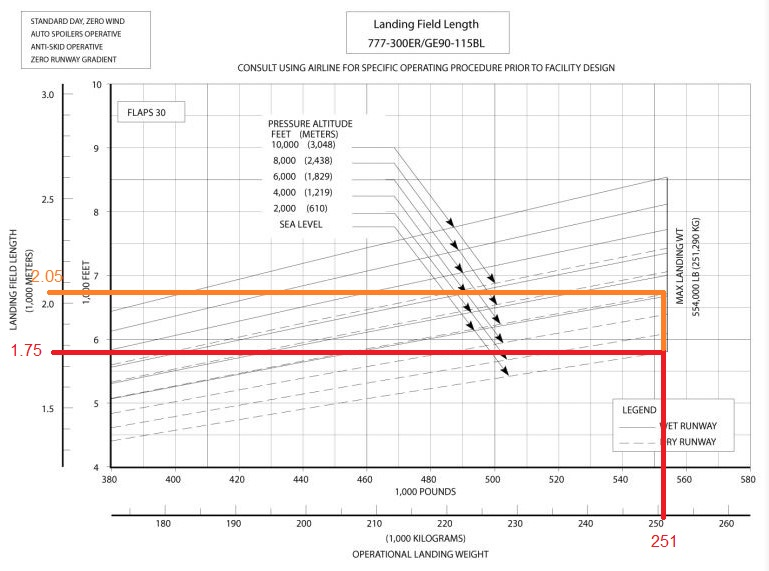
\includegraphics[clip, trim=0cm 0cm 0cm 0cm, width=0.95\textwidth]{./images/B777/landingdistance777}
	\caption{Landing distance vs MTOW for the Boeing 777.} %nom de la figura
	\label{} %per denotar una referencia
\end{figure}


TABLE
\begin{table}[htb]
	\centering
	\begin{tabular}{ll p{5cm}}
		\midrule[2pt]
		\(T_1\)& 13 cm\\
		\(T_2\) & 21 cm\\
		\(T_3\)& 62 cm \\
		\(T_t\)& 95 cm\\
		\bottomrule[2pt]
	\end{tabular}
	\caption{Thickness after the materials correction factor.}
	\label{}
\end{table}
\chapter{Aim}
\paragraph{} This projects aims to compute an interplanetary trajectory which, for a given ecliptic rectangular positions of two planets in two known time instances, is able to carry a spaceship with a unique impulse, from the first planet to the second.

\chapter{Theoretical background}



\section{Planetary orbits and approximations analysis}
In order to calculate the interplanetary trajectory between two planets, several approximations can be used. The simplest approximation, which can be called \textit{aprox. 0} accepts the following hypothesis: 
\begin{itemize}
\item Circular and coplanar orbits
\item No analysis about the exit of the planet of start is done.
\item No analysis about entering the planet of arrival is done. 
\end{itemize} 
\textit{Aprox. 0} is very basic and can be easily improved adding some parameters.\\
Another approximation widely used is \textbf{Patched Conic Approximation (PCA)}. This method improves significantly the results obtained with \textit{aprox. 0} and represents a good starting point for a more precise numerical analysis of the mission. For this reason, in this project the PCA method will be used. 
\subsection{Patched Conic Approximation (PCA)}
The Patched Conic Approximation (PCA) consist on the evaluation of an interplanetary trajectory dividing it into three stages. Considering the Earth as the planet of start, this stages are: 
\begin{itemize}
\item Geocentric phase: Hyperbolic exit of the Earth. This phase takes place while the probe is going through the influence sphere of the Earth. 
\item Heliocentric phase: Elliptic trajectory with the Sun as main influencer.
\item Planet-centred phase: Hyperbolic arrival to the planet of destination. Similarly to the geocentric phase, this phase starts when the probe enters the sphere of influence of the planet. 
\end{itemize}
The influence spheres mentioned are the space close to the planets where it can be considered that the influence of the Sun is negligible in comparison with that of the planet in question. The Laplace criteria will be considered to calculate this sphere. In Table \ref{RIplanets} the radius of the sphere of influence of the solar system's planets are shown. 
\begin{table}[H]
\centering
\begin{tabular}{|lccc|}
\hline
Planet  & $R_I\times 10^6 $km & $R_I\times 10^{-3} $ UA & $R_I$ Radius of the planet \\ \hline
Mercury & 0.111                       & 0.740                        & 45                     \\
Venus   & 0.616                       & 4.11                         & 100                    \\
Earth   & 0.924                       & 6.16                         & 145                    \\
Mars    & 0.577                       & 3.85                         & 170                    \\
Jupiter & 48.157                      & 321.0                        & 677                    \\
Saturn  & 54.796                      & 365.3                        & 901                    \\
Uranus  & 91.954                      & 346.4                        & 2025                   \\
Neptune & 80.196                      & 534.6                        & 3866                   \\ \hline
\end{tabular}
\caption{Radius of influence of the planets}
\label{RIplanets}
\end{table}
In order to set out the problem and begin with the resolution of it using the PCA method, the times and positions of the planets at the beginning and end of the trajectory are needed and some hypothesis are taken under consideration. The hypothesis are: 
\begin{itemize}
\item The spheres of influences of the planets are not considered during the heliocentric phase. This hypothesis is admissible because the radius of the sphere are very small in comparison with the distance between planets.
\item The spheres of influence are considered infinite from the point of view of the planet. This is assumed due to the fact that the radius of influence of the planets are much larger than the radious of the planet itself, as can be seen in Tabl \ref{RIplanets}.
\item The duration of the trajectory can be taken as the duration of the heliocentric phase. 
\end{itemize}
 With this data the trajectory can be found through the orbital elements of the trajectories and the thrust required. 

\subsubsection{1st. Geocentric stage }
This first stage of the trajectory of the probe aims to escape the gravitational field exerted by the departure planet. To achieve this, it is necessary to follow a hyperbolic trajectory that guarantees to pass through the planet sphere of influence with a relative velocity $V_\infty$ (also known as hyperbolic excess velocity).

Therefore, in this section necessary equations to characterize this hyperbole will be reviewed. Figure~\ref{fig:HyperParam} shows the aforementioned situation. From the figure, it can be inferred that the hyperbola is defined by:
\begin{itemize}
	\item \textit{C}: Center of the hyperbola.
	\item $beta$: Angle of the hyperbola.
	\item \textit{b}: Exit parameter.
\end{itemize} 

\begin{figure}[H]
	\centering
	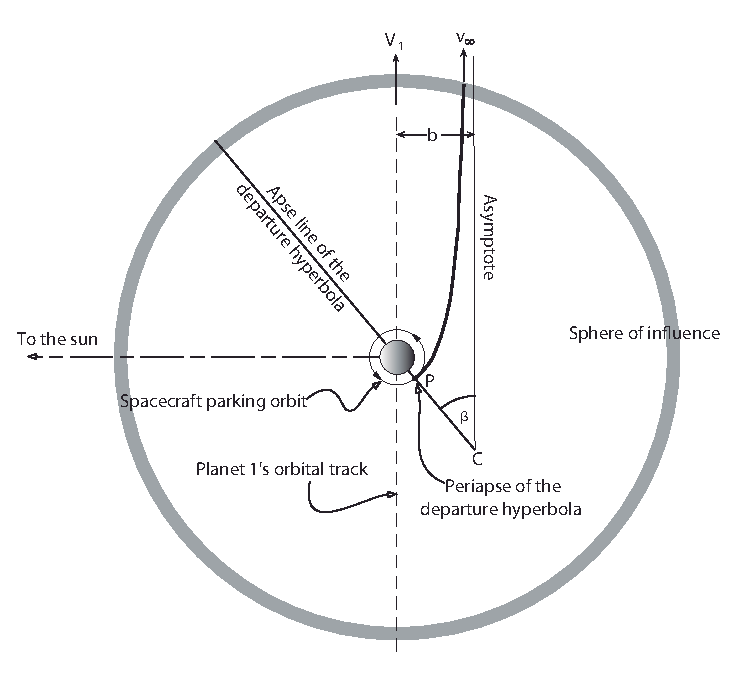
\includegraphics[width=0.5\textwidth]{././images/1stStage1} 
	\caption{Hyperbola Parameters. Extracted from~\cite{llibreVictor}.}
	\label{fig:HyperParam}
\end{figure}

The hyperbola can also be defined by the semi-major axis (\textit{a}) and the eccentricity (\textit{e}). In addition, the $\Delta V$ necessary to inject the probe into the hyperbolic orbit from the parking orbit must be specified.

To obtain these parameters, only the heliocentric departure speed ($v_1$), the velocity of the departure planet ($v_p$) and the parking orbit (in particular, the periapse radius and the speed of the orbit) are needed.


\paragraph{Definition of hyperbola:}
The first step is to obtain the semi-major axis of the hyperbola. This is obtained from the hyperbolic excess velocity as:
\begin{equation}
	a = \frac{\mu}{V_\infty^2}
\end{equation}

where $\mu$ is the standard gravitational parameter ($\mu=GM$) for the sun and the excess velocity is computed as the difference between the probe velocity and the departure planet speed. The eccentricity of hyperbola is defined by:
\begin{equation}
	e=1+(\frac{V_\infty}{V_0})^2
\end{equation}
where $V_0$ refers to the speed of the parking orbit. If this orbit is assumed to be circular with $r_0$ as the periapse, the probe velocity through the parking orbit is given by:
\begin{equation}
	V_0=\sqrt{\mu_0/r_0}
\end{equation}

being $\mu_0$ the standard gravitational parameter of the departure planet. Once the eccentricity is computed, the beta angle is easily obtained as:
\begin{equation}
	\cos \beta = \frac{1}{e}
\end{equation}

Finally, the exit parameter is computed by means of:
\begin{equation}
	b=a\sqrt{e^2-1}
\end{equation}

Obtaining the center of the hyperbola is a little bit more cumbersome. Given the three velocities ($V_\infty$, $v_p$ and $v_1$), the two frames of the figure~\ref{fig:frames} can be defined. One has the Y-axis in the direction of the planet velocity and the other has the vernal point over the X-axis. Then, the angle between the planet velocity and this X-axis is defined as $\lambda_v=90+\lambda_x$. Determining this $\lambda_x$ at the injection time $t_1$ 
allows us to obtain the right ascension ($\alpha$) and the declination ($\delta$) of the $v_1$ velocity by means of a change of frame:
\begin{equation}
	\left[\vec{V_\infty}\right]_\mathcal{Q}=\mathcal{R}_1(-\varepsilon)\mathcal{R}_3(-\lambda_x)	\left[\vec{V_\infty}\right]_\mathcal{K}
\end{equation}
Thus,
\begin{equation}
	\sin \delta =\left[V_z\right]_\mathcal{Q}; \qquad \tan \alpha=\left[\frac{V_y}{V_x}\right]_\mathcal{Q}
\end{equation}
Finally, the center of the hyperbola has the following coordinates ($\alpha+12^h$, $\delta$).
\begin{figure}[H]
	\centering
	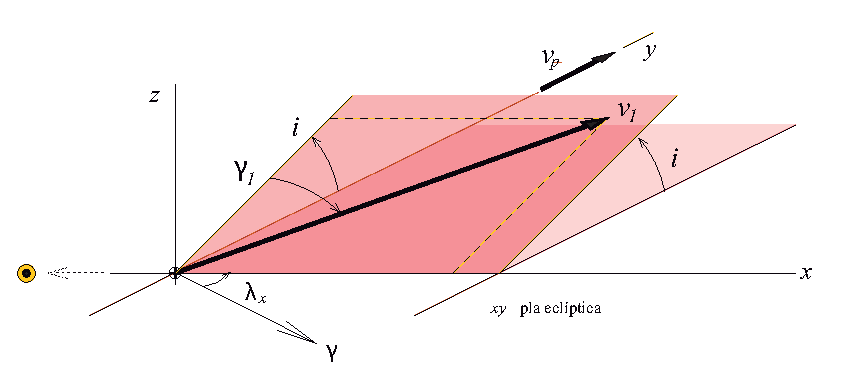
\includegraphics[width=0.5\textwidth]{././images/1stStage2} 
	\caption{Velocities frames of reference. Extracted from~\cite{PCA}}
	\label{fig:frames}
\end{figure}
\paragraph{Delta-v determination}
The necessary delta-v to put the probe onto the hyperbolic departure trajectory is given by:
\begin{equation}
	\Delta V=v_p-V_0=\sqrt{V_\infty+2V_0}-V_0
\end{equation}
The only requirement of the plane of the departure hyperbola is that it must contain the planet center of mass as well as the hyperbolic excess velocity. Therefore, the delta-v has to be applied once the probe flies over C, at a distance of $r_0*\sin \beta$. The circle of all the possible perigees is the injection points circle.
\begin{figure}[H]
	\centering
	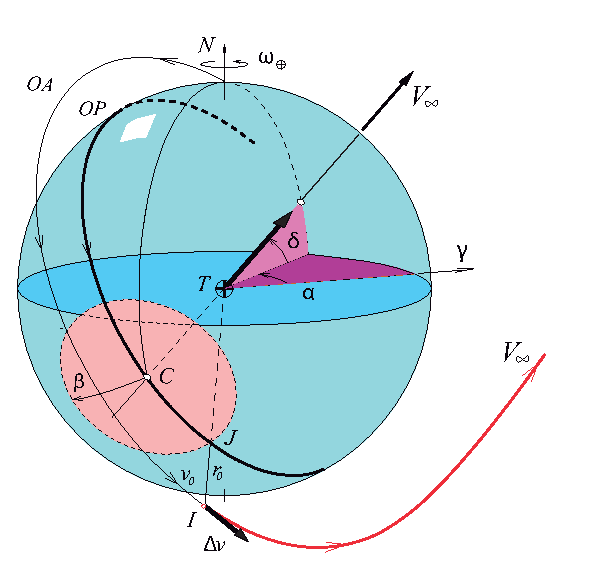
\includegraphics[width=0.5\textwidth]{././images/1stStage3} 
	\caption{Injection points circle. Extracted from~\cite{PCA}}
\end{figure}



\subsubsection{2nd. Heliocentric stage }
In this section the equations and assumptions done in order to obtain the orbital elements of the trajectory will be explained. The objective of the calculations done regarding this stage is to find:
\begin{itemize}
\item $\Omega$ : Right ascension of the ascending node.
\item \textit{e}: Eccentricity.
\item \textit{i}: Inclination to the ecliptic plane.
\item \textit{a}: Semimajor axis.
\item $\omega$ : Argument of the perihelion. 
\end{itemize} 
As said previously, the times of departure and arrival are provided, together with the position of the planets. The steps to be followed to achieve the aim of this section are now explained.
\paragraph{Longitude, latitude and distance}
The position vector is defined as: 
\begin{equation}
\overrightarrow{r}=\left( x_k, y_k, z_k \right)
\end{equation}
Where: 
\begin{equation}
x_k = r cos\beta cos\lambda
\end{equation}
\begin{equation}
y_k=r cos\beta sin\lambda
\end{equation}
\begin{equation}
z_k=r sin\beta
\end{equation}
Then longitude, latitude and distance are computed with: 
\begin{equation}
r=|\overrightarrow{r}|
\end{equation}
\begin{equation}
\beta = \arcsin\left(\frac{z_k}{r}\right)
\end{equation}
\begin{equation}
\lambda = \arctan\left(\frac{y_k}{x_k}\right)
\end{equation}
The difference between $\lambda$ at the beginning and at the end of the trajectory is an important magnitude that will be used. Taking into account that subscript 1 refers to the start position and subscript 2 to the end: 
\begin{equation}
\Delta \lambda = \lambda _2 - \lambda _1
\end{equation}
\paragraph{Inclination, right ascension of the ascending node and true anomaly variation}
Trigonometry has to be used to compute this elements. A general case will be considered, that is to say, that no assumption will be done on whether the two planets are on the ecliptic or not. As shown in reference \cite{PCA}, the equations to be used are: 
\begin{equation}
\cos \Delta\theta = \sin\beta _1 \sin\beta _2 + \cos\beta _1 \cos\beta _2 \cos\Delta\lambda
\end{equation} 
\begin{equation}
\sin A=\cos\beta _2 \frac{\sin\Delta\lambda}{\sin\Delta\theta}
\end{equation}
\begin{equation}
\cos i=\sin A\cos\beta_1
\end{equation}
\begin{equation}
\sin l=\frac{\tan\beta _1}{\tan i}
\end{equation}
\begin{equation}
\tan \sigma = \frac{\tan \beta _1}{\cos A}
\end{equation}
\begin{equation}
\Omega = \lambda _1-l
\end{equation}
\paragraph{Eccentricity, semimajor axis and true anomaly of the starting point}
With the aim of obtaining this data three equations can be stated. Due to the complexity of the equations, the resolution will be done iteratively. Two cases will be considered: elliptic and hyperbolic. Its equations and iteration process are now shown: 
\begin{itemize}
\item Elliptic trajectory:
The equations of the elliptic trajectory are: 
\begin{equation}
e=\frac{r_2-r_1}{r_1\cos\theta _1-r_2\cos(\theta_1+\Delta\theta)}
\end{equation}
\begin{equation}
a=\frac{r_1\left(1+e\cos\theta _1\right)}{1-e^2}
\end{equation}
\begin{multline}
t_2-t_1=\frac{365.25}{2\pi}a^\frac{3}{2}\Bigg(2\arctan\bigg(\sqrt{\frac{1-e}{1+e}}\tan\frac{\theta _1 +\Delta\theta}{2}\bigg)\\-\frac{e\sqrt{1-e^2}\sin (\theta _1+\Delta\theta)}{1+e\cos (\theta _1+\Delta\theta}-2\arctan\bigg(\sqrt{\frac{1-e}{1+e}}\tan \frac{\theta _1}{2}\bigg)+\frac{e\sqrt{1-e^2}\sin \theta _1}{1+e\cos \theta1}\Bigg)
\end{multline}

The iteration process done to solve the equations will deal with the difference between the time of the mission calculated and the real time of the mission, that is a known value. An error criteria $\epsilon$ is defined as the convergence value. Since the convergence criteria gives a difference in terms of time and the tuning parameter is an angle, there is no possibility to develop an adaptive increase step for $\theta_1$ (due to their completely different physical meaning). However, a kind of \textit{intelligent} convergence can be applied involving the sign of the time difference multiplying the $\theta$ step by the time error and dividing it by the time error absolute value.

Another issue related to the algorithm based on tuning an angle is the possibility of entering into a loop between two results if the step used is not small enough. To solve this problem, the algorithm includes a procedure to detect this situation and reduce the $\theta$ step in order to avoid the loop. The flow chart of this iteration (without the details of the aforementioned convergence system) is shown in Figure \ref{Floweliptic}.
\begin{figure}[H]
\centering
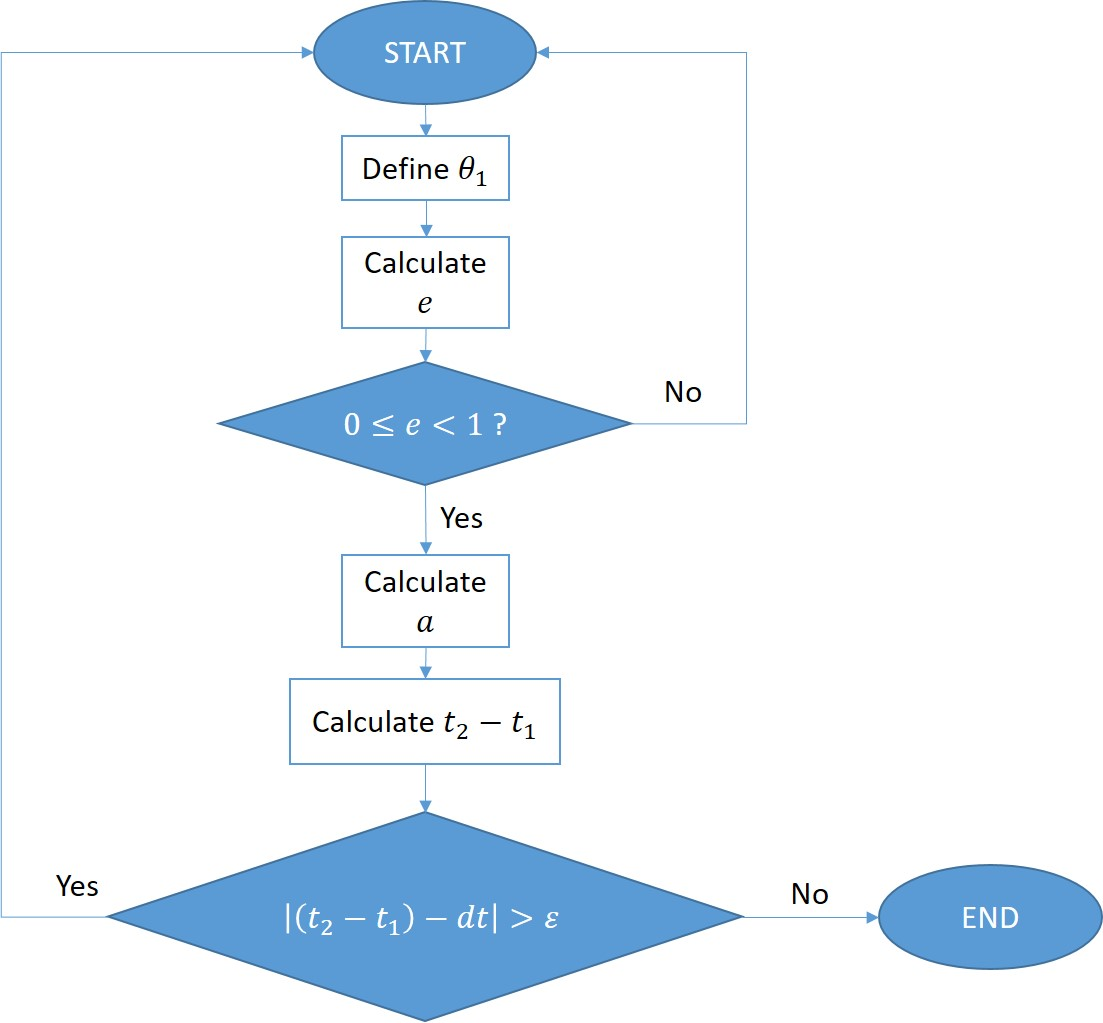
\includegraphics[width=0.8\textwidth]{././images/flowcharteliptic.jpg} 
\caption{Flow chart for the elliptic trajectory resolution.}
\label{Floweliptic}
\end{figure}
\item Hyperbolic trajectory: The equations of the hyperbolic trajectory are:
\begin{equation}
e=\frac{r_2-r_1}{r_1\cos\theta _1-r_2\cos(\theta_1+\Delta\theta)}
\end{equation}
\begin{equation}
a=\frac{r_1\left(1+e\cos\theta _1\right)}{e^2-1}
\end{equation}
\begin{multline}
t_2-t_1=\frac{365.25}{2\pi}a^\frac{3}{2}\Bigg( \frac{e\sqrt{e^2-1}\sin (\theta _1 +\Delta\theta)}{1+e\cos (\theta _1+\Delta\theta)} - \\
ln \left| \frac{\tan \frac{\theta _1 +\Delta\theta}{2}+\sqrt{\frac{e+1}{e-1}}}{\tan \frac{\theta _1 +\Delta\theta}{2} -\sqrt{\frac{e+1}{e-1}}} \right| -\frac{e\sqrt{e^2-1}\sin \theta _1}{1+e\cos \theta _1}+ln\left| \frac{\tan \frac{\theta _1}{2}+\sqrt{\frac{e+1}{e-1}}}{\tan \frac{\theta _1}{2}-\sqrt{\frac{e+1}{e-1}}}\right| \Bigg)
\end{multline}
The resolution is similar to that of the elliptic case, but the acceptable values of the eccentricity change. The flow chart is shown in Figure \ref{Flowhyp}.
\begin{figure}[H]
\centering
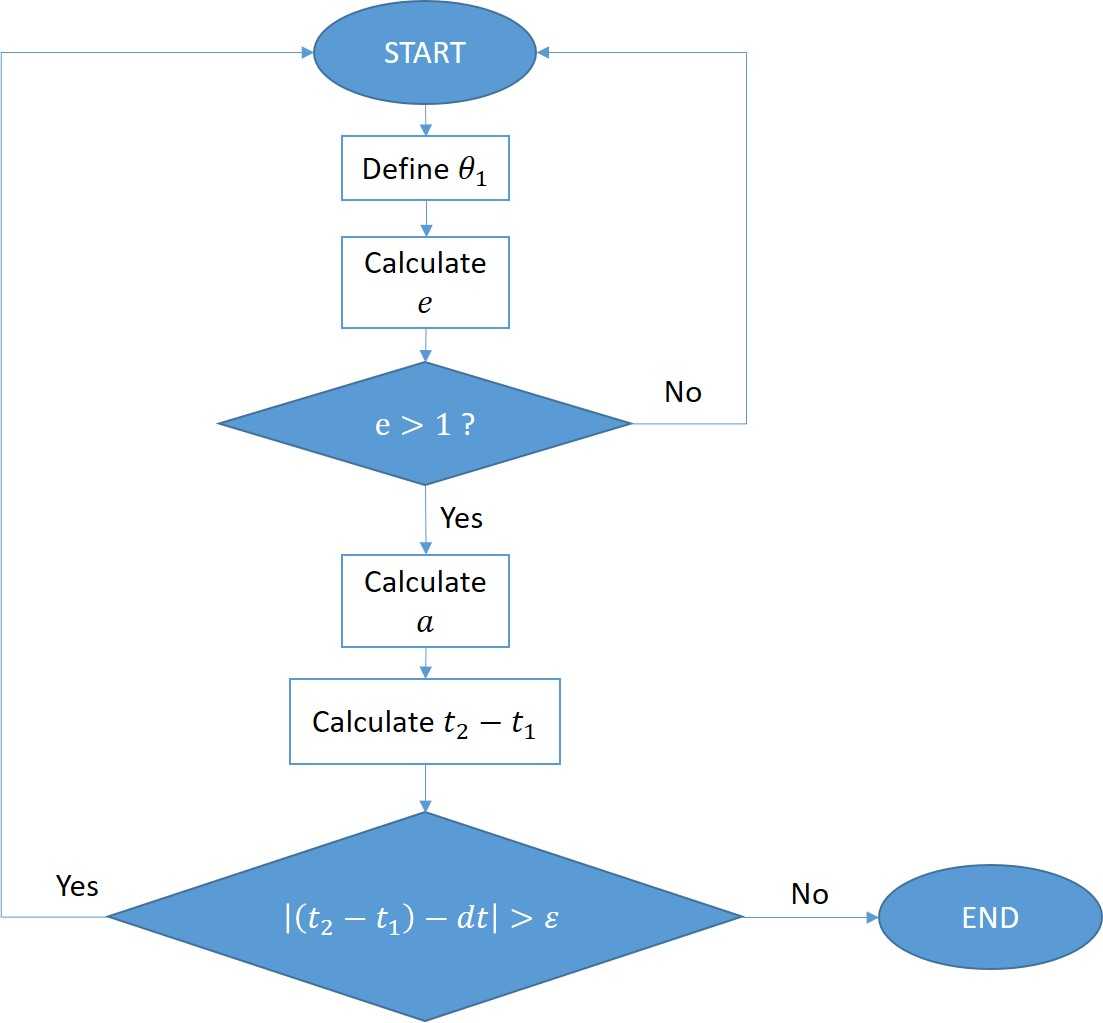
\includegraphics[width=0.8\textwidth]{././images/flowcharthyp.jpg} 
\caption{Flow chart for the hyperbolic trajectory resolution.}
\label{Flowhyp}
\end{figure}
\end{itemize}
\paragraph{Argument of the perihelion} 
The only remaining orbit element that needs to be computed is $\omega$. It can be calculated using results from the previous steps:
\begin{equation}
\omega = 2\pi - (\theta _1 - \sigma )
\end{equation}



\subsubsection{3rd. Planetocentric stage }
\paragraph{} Once the spacecraft, enter into the SOI of the destination planet, the planetocentric stage starts. The spacecraft, describes a planet arrival hyperbola. Depending of the arrival velocity and position three main scenarios can be described for the spacecraft.

\begin{description}
	\item[Impact] If arrival position $r_p \leq R_P$.
	\item[Slowdown] Atmosphere interaction will slowdown the spacecraft if $r_p \leq R_a$.
	\item[Flyby] Spacecraft will perform a flyby over the planet if $r_p > R_a$ or $b > b_a$.	
\end{description}

Note that $R_P$ and $R_a$, correspond to the planet and atmosphere radius respectively.

The spacecraft, will only stay trapped on the destination planet, orbiting, if the spaceship has slowdown enough in contact with the planet atmosphere or the spaceship braked during the periastron.

Because, the main assignment objective was to calculate, a trajectory between to planets for interplanetary travel. This stage is been only develop theoretically, expressions for computing theses parameters can be obtained on, \cite{PCA}. First and third stage of the PCA, share some concepts and equations because in both, an hyperbolic trajectory is performed.  
\chapter{Calculations and results}

\section{Verification}
In order to verify the code, examples shown at reference \cite{CalafEnunciat} will be used. In this section, the results provided for every example will be exposed together with the results obtained using the code developed for this project and conclusions will be extracted.
\subsection{From Earth to Mars using an elliptic heliocentric trajectory}
\begin{table}[H]
\centering
\begin{tabular}{|lc|}
\hline
Departure date              & 2020 Jul 19                \\ 
Arrival date                & 2021 Gen 25                \\ 
$\Delta$t                    & 190 days                   \\ 
$r_1$                          & (0.4537, -0.9094, 0.0000)AU  \\ 
$r_2$                          & (0.3148, 1.5078, 0.0239)AU   \\ \hline
\end{tabular}
\caption{Data provided by the first example}
\end{table}

\begin{table}[H]
\centering
\begin{tabular}{|lc|}
\hline
Semimajor axis                          & 1.33069 AU      \\ 
Eccentricity                           & 0.23629         \\ 
$\theta _0$                     & 359.621\degree                 \\ 
$\omega$                           & 0.470\degree                                 \\ 
Inclination                          & 1.435\degree                             \\ 
$\Omega$                & 296.424º                   \\ 
Heliocentric velocity at departure (km/s) & (29.3678, 14.6982, 0.8229) \\ 
Heliocentric velocity at arrival (km/s) & (20.4069,8.2271,0.3656)    \\
\hline
\end{tabular}
\caption{Results provided by the first example}
\end{table}

\begin{table}[H]
\centering
\begin{tabular}{|lc|}
\hline
Semimajor axis                          & 1.33073 AU      \\ 
Eccentricity                           & 0.236291         \\ 
$\theta _0$         & 359.613\degree                   \\
$\omega$                           & 0.386861\degree                            \\ 
Inclination                          & 1.43388\degree                             \\ 
$\Omega$                & 296.515\degree                                   \\ 
Heliocentric velocity at departure (km/s) & (29.367,14.6986,0.822024) \\ 
Heliocentric velocity at arrival (km/s)&   (-20.4068,8.27743,-0.364583) \\
\hline
\end{tabular}
\caption{Results computed by the code developed for the first example}
\end{table}


\begin{table}[H]
\centering
\begin{tabular}{|cc|}
\hline
\textbf{Parameter}   & \textbf{Relative error (\%)} \\ \hline
a           & 0.0030              \\
e           & 0.0004              \\
$\theta _0$ & 0.0022              \\
$\omega$    & 17.6891              \\
i           & 0.0780              \\
$\Omega$    & 0.0307              \\
$v_{t_1}$   & 0.0017              \\
$v_{t_1}$   & 0.0001              \\ \hline
\end{tabular}
\caption{Relative error in the first example}
\end{table}

\subsection{From Mars to Jupiter using an elliptic heliocentric trajectory}
\begin{table}[H]
\centering
\begin{tabular}{|lc|}
\hline
Departure date              & 2026 Jun 05                \\ 
Arrival date                & 2029 April 25                \\ 
$\Delta$t                    & 1055 days                   \\ 
$r_1$                          & (1.3277, 0.4901, 0.0223)AU  \\ 
$r_2$                          & (5.0135, 2.1380, 0.0505)AU   \\ \hline
\end{tabular}
\caption{Data provided by the second example}
\end{table}


\begin{table}[H]
\centering
\begin{tabular}{|lc|}
\hline
Semimajor axis                          & 3.45403 AU      \\ 
Eccentricity                           & 0.59218         \\ 
$\theta _0$                     & 350.769\degree                 \\ 
$\omega$                           & 182.312\degree                                 \\ 
Inclination                          & 7.513\degree                             \\ 
$\Omega$                & 207.121º                   \\ 
Heliocentric velocity at departure (km/s) & (12.5324, 28.6817, 4.1200) \\ 
Heliocentric velocity at arrival (km/s) & (1.9715,7.9799,1.0552)    \\
\hline
\end{tabular}
\caption{Results provided by the second example}
\end{table}

\begin{table}[H]
\centering
\begin{tabular}{|lc|}
\hline
Semimajor axis    &  3.45405    \\ 
Eccentricity       & 0.592181        \\ 
$\theta _0$                &     350.469\degree \\
$\omega$             & 196.156\degree                            \\ 
Inclination                          & 7.508444\degree                             \\ 
$\Omega$          & 207.127\degree                                   \\ 
Heliocentric velocity at departure (km/s) & (-19.0894,24.8148,-4.05809)\\ 
Heliocentric velocity at arrival (km/s)&    (3.83725,-7.26513,1.08284)\\
\hline
\end{tabular}
\caption{Results computed by the code developed for the second example}
\end{table}

\begin{table}[H]
\centering
\begin{tabular}{|cc|}
\hline
\textbf{Parameter}   & \textbf{Relative error (\%)} \\ \hline
a           & 0.0006              \\
e           & 0.0002              \\
$\theta _0$ & 0.0000              \\
$\omega$    & 7.5936              \\
i           & 0.0606              \\
$\Omega$    & 0.0029              \\
$v_{t_1}$   & 0.0014              \\
$v_{t_1}$   & 0.0001              \\ \hline
\end{tabular}
\caption{Relative error in the second example}
\end{table}

\subsection{From Earth to Mars using an hyperbolic heliocentric trajectory}

\begin{table}[H]
\centering
\begin{tabular}{|lc|}
\hline
Departure date              & 2020 Mar 06                \\ 
Arrival date                & 2020 Jun 09 \\ 
$\Delta$t                    & 95 days                   \\ 
$r_1$                          & (-0.9609, 0.2466, 0.0000)AU  \\ 
$r_2$                          & (0.7285, -1.1980,-0.0430)AU   \\ \hline
\end{tabular}
\caption{Data provided by the third example}
\end{table}

\begin{table}[H]
\centering
\begin{tabular}{|lc|}
\hline
Semimajor axis         & 71.08581 AU      \\ 
Eccentricity                           & 1.01113         \\ 
$\theta _0$                     & -53.310\degree                 \\ 
$\omega$                           & 233.297\degree                                 \\ 
Inclination                          & 2.513\degree                             \\ 
$\Omega$                & 345.619º                   \\ 
Heliocentric velocity at departure (km/s) & (9.1364, -41.4090, -1.6612) \\ 
Heliocentric velocity at arrival (km/s) & (35.1754,-6.3201,0.1148)    \\
\hline
\end{tabular}
\caption{Results provided by the third example}
\end{table}

\begin{table}[H]
\centering
\begin{tabular}{|lc|}
\hline
Semimajor axis       &   71.6165   \\ 
Eccentricity              & 1.01105       \\ 
$\theta _0$      &   306.691\degree      \\
$\omega$            & 233.309\degree                            \\ 
Inclination                & 2.51416\degree                             \\ 
$\Omega$            & 345.607\degree                                   \\ 
Heliocentric velocity at departure (km/s) & (9.13562,-41.4082,-1.66139)\\ 
Heliocentric velocity at arrival (km/s)&    (35.1747,-6.31841,0.115199)\\
\hline
\end{tabular}
\caption{Results computed by the code developed for the third example}
\end{table}

\begin{table}[H]
\centering
\begin{tabular}{|cc|}
\hline
\textbf{Parameter}   & \textbf{Relative error (\%)} \\ \hline
a           & 0.7465              \\
e           & 0.0079              \\
$\theta _0$ & 0.0003              \\
$\omega$    & 0.0051              \\
i           & 0.0462              \\
$\Omega$    & 0.0035              \\
$v_{t_1}$   & 0.1189              \\
$v_{t_1}$   & 0.0028              \\ \hline
\end{tabular}
\caption{Relative error in the third example}
\end{table}
\subsection{Verification conclusions}
It can be appreciated that in most of the cases the relative error is far less than one. The highest error produced is less than 17\%, and its cause probably deal with the equations and assumptions done while computing the results.

Although, heliocentric arrival and departure velocities, may differ in some sign for one of the components. After an extensive study, is determined that could be, because of the angles definition. This opposite values, show that the vector obtained is just the symmetric, that is equivalent to the solution if angles are chosen accordingly

Therefore, the code is taken as valid and can be used in order to obtain other interplanetary trajectories. It has been designed in a general manner so the same code can compute elliptic and hyperbolic trajectories with any departure and arrival planet in the solar system. 

\section{Main interplanetary orbit calculations}
Following, the cases proposed in reference \cite{CalafEnunciat} will be solved. 
\subsection{Case 1: Mars to Jupiter}

\begin{table}[H]
\centering
\begin{tabular}{|lc|}
\hline
Departure date              & 2037 Oct 25                \\ 
Arrival date                & 2039 Oct 15 \\ 
$\Delta$t                    & 720 days                   \\ 
$r_1$                          & (1.0707, 0.9868, 0.0055)  \\ 
$r_2$                          & (5.2210, 1.4357,0.1109)   \\ \hline
\end{tabular}
\caption{Data provided for a travel between Mars and Jupiter}
\end{table}

\begin{table}[H]
\centering
\begin{tabular}{|lc|}
\hline
Semimajor axis       &  4.27012 AU  \\ 
Eccentricity         &    0.725509   \\ 
$\theta _0$      &  302.422 \degree      \\
$\omega$            & 63.3568\degree                            \\ 
Inclination        & 2.14985\degree                             \\ 
$\Omega$        & 36.89\degree                                   \\ 
Heliocentric velocity at departure (km/s) & (-29.1352,12.6808,1.03727) \\ 
Heliocentric velocity at arrival (km/s)&    (4.72014,-9.86931,-0.402679)\\
\hline
\end{tabular}
\caption{Results computed for a travel between Mars and Jupiter}
\end{table}

\subsection{Case 2: Earth to Mars}

\begin{table}[H]
\centering
\begin{tabular}{|lc|}
\hline
Departure date              & 2033 Mar 13                \\ 
Arrival date                & 2033 Aug 05 \\ 
$\Delta$t                    & 145 days                   \\ 
$r_1$                          & (0.9848, 0.1338, 0.0000)  \\ 
$r_2$                          & (0.6797, 1.2298,0.0424)   \\ \hline
\end{tabular}
\caption{Data provided for case 2}
\end{table} 

\begin{table}[H]
\centering
\begin{tabular}{|lc|}
\hline
Semimajor axis     & 1.37053 AU \\ 
Eccentricity        &    0.615632   \\ 
$\theta _0$    &   256.507\degree      \\
$\omega$        & 103.493\degree                            \\ 
Inclination         & 2.15438\degree                             \\ 
$\Omega$            & 7.73712\degree                                   \\ 
Heliocentric velocity at departure (km/s) & (-22.8707,24.7746,1.03934)\\ 
Heliocentric velocity at arrival (km/s)&    (9.73264,-22.7879,-0.898741)\\
\hline
\end{tabular}
\caption{Results computed for case 2}
\end{table}
\subsection{Case 3: Earth to Mars}
\begin{table}[H]
\centering
\begin{tabular}{|lc|}
\hline
Departure date              & 2031 Jan 23                \\ 
Arrival date                & 2031 Aug 01 \\ 
$\Delta$t                    & 190 days                   \\ 
$r_1$                          & (0.5264, 0.8316, 0.0001)  \\ 
$r_2$                          & (0.0108, 1.4542,0.0309)   \\ \hline
\end{tabular}
\caption{Data provided for case 3}
\end{table}

\begin{table}[H]
\centering
\begin{tabular}{|lc|}
\hline
Semimajor axis       &  1.24706 AU
   \\ 
Eccentricity              &   0.381113
    \\ 
$\theta _0$      &  282.584
 \degree      \\
$\omega$            & 77.5612
\degree                            \\ 
Inclination                & 2.29274
\degree                             \\ 
$\Omega$            & 57.8117
\degree                                   \\ 
Heliocentric velocity at departure (km/s) & (-48.5598,30.3938,2.29362) \\ 
Heliocentric velocity at arrival (km/s)&   (20.646,-0.03366,-0.70028) \\
\hline
\end{tabular}
\caption{Results computed for case 3}
\end{table}
\subsection{Case 4: Earth to Mars}

\begin{table}[H]
\centering
\begin{tabular}{|lc|}
\hline
Departure date              & 2025 Jul 18                \\ 
Arrival date                & 2025 Oct 21 \\ 
$\Delta$t                    & 95 days                   \\ 
$r_1$                          & (0.4342, 0.9188, 0.0001)  \\ 
$r_2$                          & (0.6775, 1.3571,0.0118)   \\ \hline
\end{tabular}
\caption{Data provided for case 4}
\end{table}

\begin{table}[H]
\centering
\begin{tabular}{|lc|}
\hline
Semimajor axis       &  122.519 AU   \\ 
Eccentricity              &       -1.0008\\ 
$\theta _0$      &   360.052\degree      \\
$\omega$            & -0.0356\degree                            \\ 
Inclination                & 19.6087\degree                             \\ 
$\Omega$            & 64.7217\degree                                   \\ 
Heliocentric velocity at departure (km/s) & -\\ 
Heliocentric velocity at arrival (km/s)&    -\\
\hline
\end{tabular}
\caption{Results computed for case 4}
\end{table}
Results partially converged. Code, doesn't perform well in this case.
\subsection{Case 5: Earth to Venus}
 \begin{table}[H]
\centering
\begin{tabular}{|lc|}
\hline
Departure date              & 2023 May 27                \\ 
Arrival date                & 2023 Nov 01 \\ 
$\Delta$t                    & 158 days                   \\ 
$r_1$                          & (-0.4255, -0.9194, 0.0000)  \\ 
$r_2$                          & (0.0356, 0.7189,0.0079)   \\ \hline
\end{tabular}
\caption{Data provided for case 5}
\end{table}

\begin{table}[H]
\centering
\begin{tabular}{|lc|}
\hline
Semimajor axis       &   217.426 AU
  \\ 
Eccentricity              &   -0.847689
    \\ 
$\theta _0$      & 360.007
  \degree      \\
$\omega$            & -0.00657141
\degree                            \\ 
Inclination                & 1.67824
\degree                             \\ 
$\Omega$            & 245.165
\degree                                   \\ 
Heliocentric velocity at departure (km/s) & (2.45241,-1.13498,0.0791754) \\ 
Heliocentric velocity at arrival (km/s)&  (4.80202,-5.12288,0.190725) \\
\hline
\end{tabular}
\caption{Results computed for case 5}
\end{table}
\subsection{Case 6: Mars to Earth}

\begin{table}[H]
\centering
\begin{tabular}{|lc|}
\hline
Departure date              & 2033 Jan 18                \\ 
Arrival date                & 2033 Aug 28 \\ 
$\Delta$t                    & 222 days                   \\ 
$r_1$                          & (1.5831, 0.3913, 0.0306)  \\ 
$r_2$                          & (0.9123, 0.4340,0.0000)   \\ \hline
\end{tabular}
\caption{Data provided for case 6}
\end{table}
 
\begin{table}[H]
\centering
\begin{tabular}{|lc|}
\hline
Semimajor axis       &  1.31867 AU
   \\ 
Eccentricity              &     0.236873
  \\ 
$\theta _0$      &   180
\degree      \\
$\omega$            & 371.607
\degree                            \\ 
Inclination                & 5.3505
\degree                             \\ 
$\Omega$            & 205.441
\degree                                   \\ 
Heliocentric velocity at departure (km/s) & (-6.43846,8.513846,-0.97904) \\ 
Heliocentric velocity at arrival (km/s)&   (32.4436,-28.4563,3.71199) \\
\hline
\end{tabular}
\caption{Results computed for case 6}
\end{table}
\subsection{Case 7: Mars to Earth}

\begin{table}[H]
\centering
\begin{tabular}{|lc|}
\hline
Departure date              & 2030 Nov 20                \\ 
Arrival date                & 2031 Jul 06 \\ 
$\Delta$t                    & 228 days                   \\ 
$r_1$                          & (1.4166, 0.8722, 0.0530)  \\ 
$r_2$                          & (0.2345, 0.9893,0.0001)   \\ \hline
\end{tabular}
\caption{Data provided for case 7}
\end{table}

\begin{table}[H]
\centering
\begin{tabular}{|lc|}
\hline
Semimajor axis       &  1.30864 AU
   \\ 
Eccentricity              &   0.271869
    \\ 
$\theta _0$      &  180
 \degree      \\
$\omega$            &405.199
 \degree                            \\ 
Inclination                & 2.57215
\degree                             \\ 
$\Omega$            & 256.79
\degree                                   \\ 
Heliocentric velocity at departure (km/s) &(-9.20594,-5.75652,-0.343519) \\ 
Heliocentric velocity at arrival (km/s)&   (0.111769
,0.4865
,-0.000106258
) \\
\hline
\end{tabular}
\caption{Results computed for case 7}
\end{table}

\subsection{Case 8: Earth to Mars (hyperbolic)}
 \begin{table}[H]
\centering
\begin{tabular}{|lc|}
\hline
Departure date              & 2021 Nov 26                \\ 
Arrival date                & 2022 Feb 19 \\ 
$\Delta$t                    & 85 days                   \\ 
$r_1$                          & (0.4383, 0.8843, 0.0000)  \\ 
$r_2$                          & (-0.2082, -1.4582,-0.0255)   \\ \hline
\end{tabular}
\caption{Data provided for case 8}
\end{table}

\begin{table}[H]
\centering
\begin{tabular}{|lc|}
\hline
Semimajor axis       &  1.34023 AU
   \\ 
Eccentricity              &  1.44255
     \\ 
$\theta _0$      &   288.925
\degree      \\
$\omega$            &251.075
 \degree                            \\ 
Inclination                &3.16587
 \degree                             \\ 
$\Omega$            & 243.635
\degree                                   \\ 
Heliocentric velocity at departure (km/s) &(0.322509
, 0.650683
,0
)\\ 
Heliocentric velocity at arrival (km/s)&   (-1.20802
,-1.22481
,-0.0297817
) \\
\hline
\end{tabular}
\caption{Results computed for case 8}
\end{table}
\subsection{Case 9: Earth to Mars (hyperbolic)}

\begin{table}[H]
\centering
\begin{tabular}{|lc|}
\hline
Departure date              & 2022 Jan 15                \\ 
Arrival date                & 2022 Apr 20 \\ 
$\Delta$t                    & 95 days                   \\ 
$r_1$                          & (-0.4079, 0.8950, 0.0000)  \\ 
$r_2$                          & (0.6393, -1.2542,-0.0420)   \\ \hline
\end{tabular}
\caption{Data provided for case 9}
\end{table}

\begin{table}[H]
\centering
\begin{tabular}{|lc|}
\hline
Semimajor axis       &  5.10169 AU
   \\ 
Eccentricity              &      1.11068
 \\ 
$\theta _0$      &  280.991
 \degree      \\
$\omega$            & 259.009
\degree                            \\ 
Inclination                & 34.288
\degree                             \\ 
$\Omega$            & 294.501
\degree                                   \\ 
Heliocentric velocity at departure (km/s) &(-16.804
, -7.65848
,-12.5916
)\\ 
Heliocentric velocity at arrival (km/s)&   (36.9836
, 14.0711
,26.9253
)\\
\hline
\end{tabular}
\caption{Results computed for case 9}
\end{table}

\section{Complementary calculations}
	\subsection{Earth SOI scape parameters}
	\paragraph{} Applying the equations from the 1st geocentric stage, of the PCA. The first given example, Earth to Mars trip, planetary departure parameters are determined.
	
	\begin{table}[H]
		\centering
		\begin{tabular}{|lc|}
			\hline
			Departure date              & 2020 Jul 19                \\ 
			Arrival date                & 2021 Gen 25 \\ 
			$\Delta$t                    & 190 days                   \\ 
			$r_0$                          & 300 km  \\ 
			$I_{sp}$                          & 300 s  \\
			 \hline
		\end{tabular}
		\caption{Data provided for first example plus assumptions }
	\end{table}
	Note that $r_0$ is the initial circular parking orbit of the spacecraft and $I_{sp}$  is the specific impulse.
	
	\begin{table}[H]
		\centering
		\begin{tabular}{|lc|}
			\hline
			Hyperbolic excess speed, $v_\infty$              & 2.9439 km/s                \\ 
			Spacecraft speed on parking orbit, $v_c$                & 7.7298 km/s\\ 
			$\Delta$v                    & 3.5912 km/s                   \\ 
			Perigee of departure hyperbola                          & 6671 km  \\ 
			$\beta$                          & 29.1525 \textdegree \\
			Spacecraft fuel percent among total mass                          & 70.48 \%  \\
			\hline
		\end{tabular}
		\caption{Calculated parameter for the planetary scape.}
	\end{table}
	
	Spacecraft fuel percent among total mass is calculated as
	\begin{equation}
		\%m_{fuel} = 1-e^{(-\frac{\Delta v}{I_{sp}g_0})}
	\end{equation}
	and for this particular example means that the 70.48\% of the total spacecraft weight will be the fuel that will burn in order to scape the Earth SOI.
	\subsection{Launch windows computation}
\paragraph{}	For the first given example, Earth to Mars trip, same used in the previous section, the launch window is computed using the algorithm from the appendix A.2.2.
\begin{align*}
	C=(15.9199^h, 0.6188rad)  \qquad \qquad R=3.2497\cdot10^3 km
\end{align*}
C is given in equatorial coordinates.

These results are used to define the circle of injection points shown in the figure~\ref{fig:InjectionCircle}. C and R represent the center and the radius of the circle respectively. The spacecraft must pass over the circle center and the delta-v impulse has to be applied at the perimeter of the circle in order to leave the Earth sphere of influence with a correct hyperbolic excess velocity. In addition, knowing the launching site, the launch window availability time could be computed. 

This calculus is generic and could be computed for all studied cases. All parameters are extracted from the main code and planetary departure code, but the Earth heliocentric velocity is computed with \cite{llibreVictor} equations and checked with the given by NASA ephemerides.


	
\chapter{Conclusions} 



% BIBLIOGRAPHY

% styles:
%	abbrv   : [#] Initial. Surname (pages and vol. abbrev.)
% 	acm     : [#] Surname, Initial. (sc)
%	alpha   : [Abrev.yy] Name Surname
%	apalike : [Surname, yyyy] Surname, Initial 
%	ieeetr  : [#] Initial. Surname (pages and vol. ext.)
%	plain   : [#] Name Surname
%	siam    : [#] Initial. Surname (sc)
%	unsrt   : [#] Name Surname

\nocite{*}
\bibliographystyle{IEEEtran}
\bibliography{IEEEabrv,OrbitalMechanics} 

\appendix
\chapter{Developed algorithms}
All developed algorithm, had been computed with Matlab scripts. All of them, are attached together with the report, on a zip file for delivery. Following, developed algorithms concept and structure will be outlined.
	\section{Main code purpose and algorithm}
	\paragraph{} Main code implemented, \textit{Main\_HeliocentricOrbitalElements.m}, calculates the heliocentric stage related parameters of the PCA, in a generic way. The implemented algorithm is:
	\begin{enumerate}
		\item \textbf{Load input data}: Obtain departure and arrival dates, fly time in days, planets heliocentric positions for the departing day and $\mu_\odot$.
		\item \textbf{Select kind of trajectory}: Trajectory can be elliptic or hyperbolic.
		\item \textbf{Initial calculations}: Calculate $||\vec{r}||, \beta, \lambda, \Delta\lambda, \Omega, i, \sigma$.
		\item \textbf{Iterate until convergence}: Find values $e, a, \theta_1$, by iterating the functions \textit{Computeeliptic.m} for elliptic cases or \textit{Computehyperbolic.m} for hyperbolic cases.
		\item \textbf{Compute $\omega$}
		\item \textbf{Compute SOI arrival and departure velocities}: Find \textit{PQW} parameters, for making the calculation.
		
	\end{enumerate}

	\section{Secondary parameters code}
	\paragraph{} These codes have been develop parallel to the main code. They are use full for interesting interplanetary missions parameters, but they are not the main objective to develop on this assignment. That is why, they are treated apart.  
		\subsection{Hyperbolic scape geocentric velocities}
		Based on the equations described for the geocentric phase for the patched conics approximation. This code, \textit{Main\_GeneralManoeuvres.m}, computes the hyperbolic excess speed, the spacecraft speed on a parking orbit, $\Delta v$, the perigee of departure hyperbola the beta angle and the spacecraft fuel percent among total mass.
		\subsection{Launch windows}
		This functions, \textit{Main\_LaunchWindows.m}, is meant to be integrated on the main code, and for a given launching location and exceeds velocity $v_\infty$, can determine the time and azimuths where the launch window is available.


\end{document}